\documentclass[11pt,preprint, authoryear]{elsarticle}

\usepackage{lmodern}
%%%% My spacing
\usepackage{setspace}
\setstretch{1.2}
\DeclareMathSizes{12}{14}{10}{10}

% Wrap around which gives all figures included the [H] command, or places it "here". This can be tedious to code in Rmarkdown.
\usepackage{float}
\let\origfigure\figure
\let\endorigfigure\endfigure
\renewenvironment{figure}[1][2] {
    \expandafter\origfigure\expandafter[H]
} {
    \endorigfigure
}

\let\origtable\table
\let\endorigtable\endtable
\renewenvironment{table}[1][2] {
    \expandafter\origtable\expandafter[H]
} {
    \endorigtable
}


\usepackage{ifxetex,ifluatex}
\usepackage{fixltx2e} % provides \textsubscript
\ifnum 0\ifxetex 1\fi\ifluatex 1\fi=0 % if pdftex
  \usepackage[T1]{fontenc}
  \usepackage[utf8]{inputenc}
\else % if luatex or xelatex
  \ifxetex
    \usepackage{mathspec}
    \usepackage{xltxtra,xunicode}
  \else
    \usepackage{fontspec}
  \fi
  \defaultfontfeatures{Mapping=tex-text,Scale=MatchLowercase}
  \newcommand{\euro}{€}
\fi

\usepackage{amssymb, amsmath, amsthm, amsfonts}

\def\bibsection{\section*{References}} %%% Make "References" appear before bibliography


\usepackage[round]{natbib}

\usepackage{longtable}
\usepackage[margin=2.3cm,bottom=2cm,top=2.5cm, includefoot]{geometry}
\usepackage{fancyhdr}
\usepackage[bottom, hang, flushmargin]{footmisc}
\usepackage{graphicx}
\numberwithin{equation}{section}
\numberwithin{figure}{section}
\numberwithin{table}{section}
\setlength{\parindent}{0cm}
\setlength{\parskip}{1.3ex plus 0.5ex minus 0.3ex}
\usepackage{textcomp}
\renewcommand{\headrulewidth}{0.2pt}
\renewcommand{\footrulewidth}{0.3pt}

\usepackage{array}
\newcolumntype{x}[1]{>{\centering\arraybackslash\hspace{0pt}}p{#1}}

%%%%  Remove the "preprint submitted to" part. Don't worry about this either, it just looks better without it:
\makeatletter
\def\ps@pprintTitle{%
  \let\@oddhead\@empty
  \let\@evenhead\@empty
  \let\@oddfoot\@empty
  \let\@evenfoot\@oddfoot
}
\makeatother

 \def\tightlist{} % This allows for subbullets!

\usepackage{hyperref}
\hypersetup{breaklinks=true,
            bookmarks=true,
            colorlinks=true,
            citecolor=blue,
            urlcolor=blue,
            linkcolor=blue,
            pdfborder={0 0 0}}


% The following packages allow huxtable to work:
\usepackage{siunitx}
\usepackage{multirow}
\usepackage{hhline}
\usepackage{calc}
\usepackage{tabularx}
\usepackage{booktabs}
\usepackage{caption}


\newenvironment{columns}[1][]{}{}

\newenvironment{column}[1]{\begin{minipage}{#1}\ignorespaces}{%
\end{minipage}
\ifhmode\unskip\fi
\aftergroup\useignorespacesandallpars}

\def\useignorespacesandallpars#1\ignorespaces\fi{%
#1\fi\ignorespacesandallpars}

\makeatletter
\def\ignorespacesandallpars{%
  \@ifnextchar\par
    {\expandafter\ignorespacesandallpars\@gobble}%
    {}%
}
\makeatother

\newlength{\cslhangindent}
\setlength{\cslhangindent}{1.5em}
\newenvironment{CSLReferences}%
  {\setlength{\parindent}{0pt}%
  \everypar{\setlength{\hangindent}{\cslhangindent}}\ignorespaces}%
  {\par}


\urlstyle{same}  % don't use monospace font for urls
\setlength{\parindent}{0pt}
\setlength{\parskip}{6pt plus 2pt minus 1pt}
\setlength{\emergencystretch}{3em}  % prevent overfull lines
\setcounter{secnumdepth}{5}

%%% Use protect on footnotes to avoid problems with footnotes in titles
\let\rmarkdownfootnote\footnote%
\def\footnote{\protect\rmarkdownfootnote}
\IfFileExists{upquote.sty}{\usepackage{upquote}}{}

%%% Include extra packages specified by user

%%% Hard setting column skips for reports - this ensures greater consistency and control over the length settings in the document.
%% page layout
%% paragraphs
\setlength{\baselineskip}{12pt plus 0pt minus 0pt}
\setlength{\parskip}{12pt plus 0pt minus 0pt}
\setlength{\parindent}{0pt plus 0pt minus 0pt}
%% floats
\setlength{\floatsep}{12pt plus 0 pt minus 0pt}
\setlength{\textfloatsep}{20pt plus 0pt minus 0pt}
\setlength{\intextsep}{14pt plus 0pt minus 0pt}
\setlength{\dbltextfloatsep}{20pt plus 0pt minus 0pt}
\setlength{\dblfloatsep}{14pt plus 0pt minus 0pt}
%% maths
\setlength{\abovedisplayskip}{12pt plus 0pt minus 0pt}
\setlength{\belowdisplayskip}{12pt plus 0pt minus 0pt}
%% lists
\setlength{\topsep}{10pt plus 0pt minus 0pt}
\setlength{\partopsep}{3pt plus 0pt minus 0pt}
\setlength{\itemsep}{5pt plus 0pt minus 0pt}
\setlength{\labelsep}{8mm plus 0mm minus 0mm}
\setlength{\parsep}{\the\parskip}
\setlength{\listparindent}{\the\parindent}
%% verbatim
\setlength{\fboxsep}{5pt plus 0pt minus 0pt}



\begin{document}



\begin{frontmatter}  %

\title{Utilising Random Forest Algorithms to Classify Those Most Likely to Lose
Their Main Source of Income due to Lockdown- Evidence From NIDS-CRAM
Wave 1}

% Set to FALSE if wanting to remove title (for submission)




\author[Add1]{Johannes Coetsee - 19491050}
\ead{19491050@sun.ac.za - https://github.com/Coetsee}





\address[Add1]{Stellenbosch University}



\vspace{1cm}

\vspace{0.5cm}
\end{frontmatter}



%________________________
% Header and Footers
%%%%%%%%%%%%%%%%%%%%%%%%%%%%%%%%%
\pagestyle{fancy}
\chead{}
\rhead{July 2021 - Data Science 871}
\lfoot{}
\rfoot{\footnotesize Page \thepage}
\lhead{}
%\rfoot{\footnotesize Page \thepage } % "e.g. Page 2"
\cfoot{}

%\setlength\headheight{30pt}
%%%%%%%%%%%%%%%%%%%%%%%%%%%%%%%%%
%________________________

\headsep 35pt % So that header does not go over title




\hypertarget{introduction}{%
\section{\texorpdfstring{Introduction
\label{Introduction}}{Introduction }}\label{introduction}}

The purpose of this paper is to report on the implementation of a Random
Forest (RF) algorithm for a classification-type problem, namely, to
classify which individuals and households were more likely to lose their
main source of income due to the coronavirus and subsequent lockdown in
South Africa in March and April 2020.\footnote{The template for this
  report is based on that provided by Katzke
  (\protect\hyperlink{ref-Texevier}{2017}).} RF is well-suited for
classification-type problems, as

\hypertarget{data}{%
\section{\texorpdfstring{Data \label{Data}}{Data }}\label{data}}

This study utilises the first wave of the National Income Dynamics Study
- Coronavirus Rapid Mobile Survey 2020 (NIDS-CRAM) dataset, a
longitudinal telephonic household survey conducted by the Southern
Africa Labour and Development Research Unit (SALDRU) in April and May
2020. NIDS-CRAM investigates the various social and economic effects of
the national lockdown implemented in March 2020, and more broadly, the
consequences of the global pandemic on the South African population
Ingle \emph{et al.} (\protect\hyperlink{ref-nids2020}{2020}).\footnote{The
  data is publicly available at \url{https://www.datafirst.uct.ac.za/}.}

In total, the dataset consists of 21 features, reported in Table
\ref{Features} below, with 7073 observations in total. Table
\ref{Features} also reports the amount of missing values for each
feature, as well as a relevant description.\footnote{In this case, the
  survey answers `Refused', `Don't Know', Not Applicable and `Missing'
  are all defined as NAs.} The main feature of interest is `Income
Change' - a binary variable where a value of 1 indicates that the
household has lost their main source of income, whilst 2 indicates that
it has not. The question asked to respondents reads as follows: ``Has
your household lost its main source of income since the lockdown started
on 27th March?''.

\begin{table}
\begin{center}
\begin{tabular}{ |l|c|l| } 
 \hline
 Selected Features & NAs & Description \\ 
 \hline
  Income Change & 168 &  Has household lost main source of income since lockdown \\ 
  Sources Income Decreased & 376 & Did sources of household income decrease during lockdown \\
  Employed & 161 &  Employment Status \\
  Employment Type & 151 & Respondent's main form of work (0 = unemployed) \\
  Sources HH Income & 121 & Sources of household income in February \\
  Children Change & 93 & Change in number of children in house compared to pre-lockdown \\
  Province & 8 & Province currently living in now \\
  Dwelling Type & 6 & Type of dwelling, whether house, informal, traditional or other \\
  Race & 0 & Respondent's given population group \\
  Geo Type & 8 & Geography Type (derived from 2011 census) \\
  HH Income Apr & 2665 & Total household income after tax in April \\
  Moved & 8 & Whether respondent moved to another dwelling for lockdown \\
  Grant & 36 & Whether the respondent receives any kind of government grant \\
  Electricity Access & 2 & Whether dwelling has access to electricity \\
  Water Access & 5 & Whether dwelling has piped or tap water \\
  HH Size & 32 & Number of people resident (Household Size) \\
  Education & 45 & Highest school grade completed \\
  Tertiary & 9 & Has respondent successfully completed some tertiary education \\
  Age & 0 & Respondent's age in years \\
  Age Interval & 0 & Age interval (5 year intervals) \\
  Gender & 0 & Respondent's stated gender \\
  District Council & 8 & Municipal Demarcations Board District Council (from 2011 Census) \\
  \hline
\end{tabular}
\caption{Features}
\label{Features}
\end{center}
\end{table}

\hypertarget{missing-values-and-transformations}{%
\subsection*{Missing Values and
Transformations}\label{missing-values-and-transformations}}
\addcontentsline{toc}{subsection}{Missing Values and Transformations}

It is evident from \ref{Features} that missing values might be a
stumbling block for accurate analyses using this data. In particular,
the `HH Income Apr' variable has a large amount of NAs, most of which
are attributed to the `Don't Know' category on the questionnaire. In
other words, respondents reported that they did not know their exact
level of income for the month of April 2020. In order to avoid losing
information, this study imputes these missing values as well as for all
other features within the dataset. Furthermore, NAs for the `Employment
Type' feature are replaced by 0's to indicate `unemployed', as this
survey question was only asked to those who were employed. Those who
refused to respond or did not know their main form of work, were
indicated as missing and therefore imputed. Similarly, system NAs for
the `Tertiary' feature - a dummy variable indicating whether an
individual completed some form of tertiary education - was replaced by
0, or `no', as this question was only asked to those who were eligible.
Although not perfect solutions, these are fair assumptions to make in
order to include these potentially meaningful variables. Additionally,
the feature indicating in which District Council the household is
situated was transformed into a matrix of binary variables so as to
accommodate the necessary structure needed for imputation.\footnote{This
  is due to the fact that only 53 levels are allowed for factored
  variables using both the \emph{missForest} and \emph{randomForest}
  packages, whereas the District Council variable consists of 54 levels.}

The method of imputation used in this paper draws on a random forest
algorithm to impute missing values trained on the matrix of observed
values in the data. This can be done using the package \emph{missForest}
in R, which follows a two-step procedure. First, missing values are
pre-imputed using simple median replacement - where the missing value is
replaced with the median value computed on the rest of the observed data
for each continuous feature. For the categorical data type, missing
values are replaced by the most frequently occurring non-missing
value.\footnote{This process is also called Strawman imputation.}
Second, a forest is grown using multivariate splitting, where the
splitting rule is averaged only over non-missing values. Data is then
imputed by regressing each feature on all other features, thereafter
predicting missing values using the fitted forest. This process is
iterated in order to update the initial median-replaced values until the
stopping criterion - in our case, when the difference between the
previous iteration and new iteration have become larger once for each
data type - is met (Tang \& Ishwaran,
\protect\hyperlink{ref-tang2017random}{2017}).

The usage of this specific algorithm is necessitated by the nature of
the data, where features are of three different data types, namely,
categorical, numeric and continuous. Stekhoven \& Bühlmann
(\protect\hyperlink{ref-stekhoven2012missforest}{2012}) and Tang \&
Ishwaran (\protect\hyperlink{ref-tang2017random}{2017}) show that this
iterative RF imputation procedure outperforms many other widely-used
implementation methods such as, for instance, K-Nearest Neighbours (KNN)
imputation and Multivariate Imputation by Chained Equations (MICE),
especially within mixed-type data contexts. Furthermore, it inherits all
the positive characteristics attributed to random forests itself, such
as being robust to noisy data due to inherent feature selection, as well
as being simple to implement. However, it is computationally intensive,
and crucially also relies on the assumption that missing data are
Missing At Random (MAR). If not MAR, there is possibility of introduced
selection bias.\footnote{missForest is not unique in requiring this
  assumption, however.} This is deemed a permissible admission due to
the relatively low number of missing values in the dataset as a whole.
For the most problematic feature, `HH Income Apr', the imputation
strategy above is especially relevant as missing values are more likely
to be those closer to the median-income group than to, for instance, the
mode or mean incomes.

\hypertarget{methodology}{%
\section{\texorpdfstring{Methodology
\label{Meth}}{Methodology }}\label{methodology}}

\hypertarget{computing}{%
\subsection*{Computing}\label{computing}}
\addcontentsline{toc}{subsection}{Computing}

All computation was done using the Amazon Web Services' (AWS) Elastic
Compute Cloud (EC2) service, combined with the functionality of RStudio
Server. A `t2.micro' virtual machine instance was created with a public
IP address, through which RStudio Server was initiated.

Computing time -

Cloud computing is necessitated by especially the grid-searches employed
in later sections due to computing limitations on the local machine,
however, clustering was not deemed necessary due to the relatively small
size of the data.

Furthermore, parallel programming was utilised for the more
computationally intensive tasks such as missing value imputation and
parameter tuning (using the Parallel sockets approach for windows).

\hypertarget{sql}{%
\subsection*{SQL}\label{sql}}
\addcontentsline{toc}{subsection}{SQL}

SQL was used in two ways in this study. First, \emph{sqlite3} databases
were created for the separate tables entitled `nids' and `derived', and
subsequently compiled in one large database containing all features of
the raw data. This was done using SQL syntax and the function
\emph{dbConnect} within RStudio. However, using the Bash Unix shell for
Windows\footnote{Made accessible due to being a member of the Windows
  Insider Program.}, these tables were queried and data was surveyed in
order to select the relevant features necessary for the RF
implementation. Although not necessary to use SQL to this end, it is
more efficient in terms of memory usage than reading the larger datasets
directly into R's memory. After feature selection, the final dataset to
be read into R was once again compiled and collected within RStudio
using SQL syntax.

\hypertarget{algorithms}{%
\subsection*{Algorithms}\label{algorithms}}
\addcontentsline{toc}{subsection}{Algorithms}

This study compares the performance of three different classification
algorithms: 1) a random forest, 2) a simple Gradient Boosted Random
Forest, and 3)

\hypertarget{rf}{%
\subsection*{RF}\label{rf}}
\addcontentsline{toc}{subsection}{RF}

\hypertarget{gbm}{%
\subsection*{GBM}\label{gbm}}
\addcontentsline{toc}{subsection}{GBM}

\hypertarget{results}{%
\section{Results}\label{results}}

\hypertarget{model-1-random-forest}{%
\subsection{Model 1: Random Forest}\label{model-1-random-forest}}

\hypertarget{prediction-and-confusion-matrix-train-vs-test-data}{%
\subsubsection*{prediction and confusion matrix, train vs test
data}\label{prediction-and-confusion-matrix-train-vs-test-data}}
\addcontentsline{toc}{subsubsection}{prediction and confusion matrix,
train vs test data}

\hypertarget{error-rate-and-bootstrap-samples}{%
\subsubsection*{error rate and bootstrap
samples}\label{error-rate-and-bootstrap-samples}}
\addcontentsline{toc}{subsubsection}{error rate and bootstrap samples}

\hypertarget{number-of-nodes}{%
\subsubsection*{number of nodes}\label{number-of-nodes}}
\addcontentsline{toc}{subsubsection}{number of nodes}

\hypertarget{hyperparameter-tuning}{%
\subsubsection*{hyperparameter tuning}\label{hyperparameter-tuning}}
\addcontentsline{toc}{subsubsection}{hyperparameter tuning}

\hypertarget{variable-importance}{%
\subsubsection*{variable importance}\label{variable-importance}}
\addcontentsline{toc}{subsubsection}{variable importance}

\begin{figure}[H]
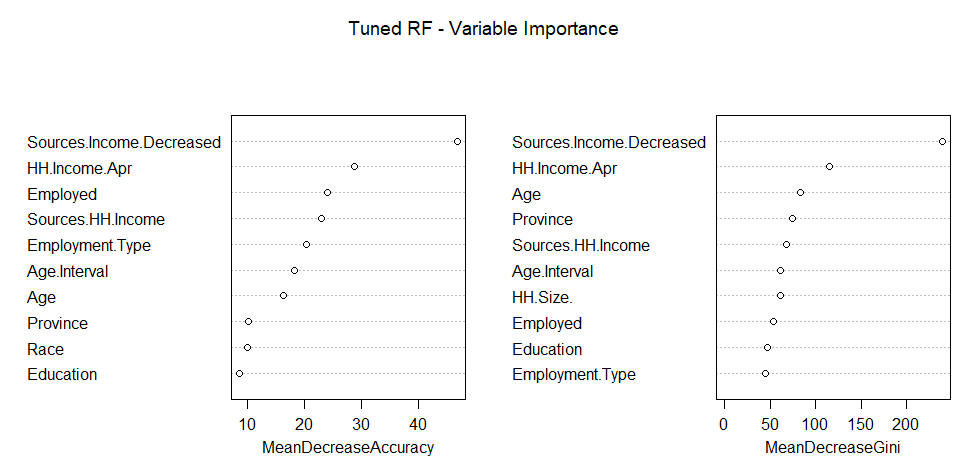
\includegraphics[width=1\linewidth]{Figures/rf3_impplot} \caption{\label{varimprf1} - RF Tuned Model}\label{fig:varimprf1}
\end{figure}

\hypertarget{mds-plots}{%
\subsubsection{MDS plots}\label{mds-plots}}

\begin{figure}[H]

{\centering 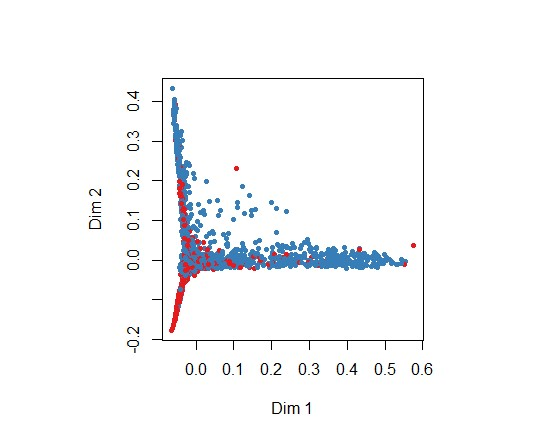
\includegraphics[width=1\linewidth,height=0.3\textheight]{Figures/MDS_rf3_train} 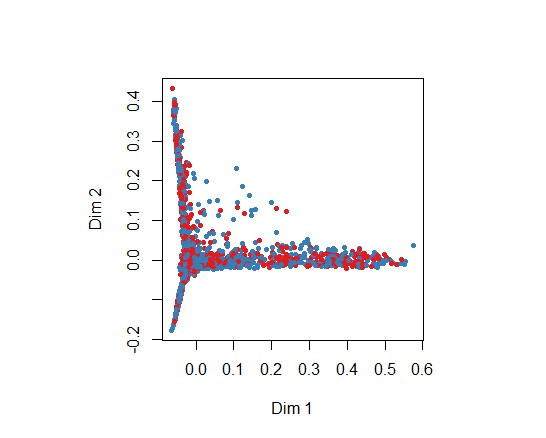
\includegraphics[width=1\linewidth,height=0.3\textheight]{Figures/MDS_rf3_test} 

}

\caption{\label{MDSrf3} - Training Data (Top), Test Data (Bottom)}\label{fig:MDSrf3}
\end{figure}

\hypertarget{model-2-gbm-random-forest}{%
\subsection{Model 2: GBM Random
Forest}\label{model-2-gbm-random-forest}}

gri

\hypertarget{conclusion}{%
\section{Conclusion}\label{conclusion}}

\newpage

\hypertarget{references}{%
\section*{References}\label{references}}
\addcontentsline{toc}{section}{References}

\hypertarget{refs}{}
\leavevmode\hypertarget{ref-nids2020}{}%
Ingle, K., Brophy, T. \& Daniels, R. 2020. National income dynamics
study--coronavirus rapid mobile survey (nids-cram) panel user manual.
\emph{Technical Note Version}. 1.

\leavevmode\hypertarget{ref-Texevier}{}%
Katzke, N.F. 2017. \emph{Texevier: Package to create elsevier templates
for rmarkdown}. ed. Stellenbosch, South Africa: Bureau for Economic
Research.

\leavevmode\hypertarget{ref-stekhoven2012missforest}{}%
Stekhoven, D.J. \& Bühlmann, P. 2012. MissForest---non-parametric
missing value imputation for mixed-type data. \emph{Bioinformatics}.
28(1):112--118.

\leavevmode\hypertarget{ref-tang2017random}{}%
Tang, F. \& Ishwaran, H. 2017. Random forest missing data algorithms.
\emph{Statistical Analysis and Data Mining: The ASA Data Science
Journal}. 10(6):363--377.

\hypertarget{appendix}{%
\section*{Appendix}\label{appendix}}
\addcontentsline{toc}{section}{Appendix}

\hypertarget{appendix-a}{%
\subsection*{Appendix A}\label{appendix-a}}
\addcontentsline{toc}{subsection}{Appendix A}

\bibliography{Tex/ref}





\end{document}
